\documentclass{lutmscthesis}[2010/09/22]
%\documentclass[draft]{lutmscthesis}   % leave figures blank, faster

\usepackage[utf8]{inputenc}
\usepackage[T1]{fontenc}
\usepackage[english]{babel}

\usepackage{times}
\usepackage{tabularx}
\usepackage{multirow}

\usepackage{setspace}
\usepackage{verbatim}
\usepackage[intlimits]{amsmath}
\usepackage{enumitem}

\usepackage{pgfplots} 
\pgfplotsset{compat=newest} 
\newlength\figurewidth
\newlength\figureheight

% Ensure figure captions are below and table captions are above the content.
\usepackage{float}
\floatstyle{plain}\restylefloat{figure}
\floatstyle{plaintop}\restylefloat{table}

\usepackage[pdfborder={0 0 0}]{hyperref}
%\usepackage[]{algorithm}
\usepackage[ruled]{algorithm2e}

\usepackage{cite}


%           Hyperref rationale - or just pain in the butt
%
% Load 'float' package first, because that will fix problems with 'algorithm'
% package interacting with hyperref.
%
% Hyperref must be the last package loaded, except...
% Load 'algorithm' AFTER hyperref, otherwise \theHalgorithm is
% undefined control sequence error appears.
%
% The TeXLive 2008 version of 'algorithmic' is buggy with hyperref.
% Use this bundled, special, hand-fixed version of algorithmic.sty
% instead. It is identified by version 2006/12/15.


\graphicspath{{resources/}}

\newcommand{\vect}[1]{\boldsymbol{#1}}
\newcommand{\matr}[1]{\boldsymbol{#1}}
\newcommand{\diag}[1]{\mathrm{diag}(#1)}
\newcommand{\iprod}[1]{\left\langle #1 \right\rangle}
\newcommand{\me}{\mathrm{e}}
\newcommand{\mi}{\mathrm{i}}
\newcommand{\md}{\mathrm{d}}
\newcommand{\sse}{{}} %\mathrm{SSE}}
\newcommand{\trace}{\mathrm{Tr}\:}
\newcommand{\frp}[2]{{}^\mathrm{#1}\vect{#2}}
\newcommand{\frs}[3]{{}^\mathrm{#1}#2_\mathrm{#3}}
\newcommand{\frv}[3]{{}^\mathrm{#1}\vect{#2}_\mathrm{#3}}
\newcommand{\frm}[3]{{}^\mathrm{#1}\matr{#2}_\mathrm{#3}}
\newcommand{\colvec}[2]{\genfrac{[}{]}{0pt}{1}{#1}{#2}}
\newcommand{\relphantom}[1]{\mathrel{\phantom{#1}}}
\newcommand\aug{\fboxsep=-\fboxrule\!\!\!\fbox{\strut}\!\!\!}

\newcommand{\etal}{\textit{et al}. }

\newtheorem{theorem}{Theorem}

% Thesis information

\title{Contour segment grouping for overlapping convex object segmentation}

\author{Nikita Ashikhmin}

\Faculty{School of Engineering Science \\ Master's Programme in Computational Engineering and Technical Physics}
\Major{Intelligent Computing Major}

\Keywords{segment grouping, convex object segmentation, concavity analysis, seed point, fast radial symmetry}

\Supervisors{
M.Sc. (Eng.) Sahar Zafari \\
Adjunct Professor, Dr. Tuomas Eerola \\
Dr. Jouni Sampo \\
Prof. Heikki Kälviäinen
}
\Examiners{Professor Heikki K\"alvi\"ainen \\Associate Professor, Cand. Sci Gleb Radchenko}

\Year{2017}

% Thesis statistics: figure, table and appendix counts, for abstracts
\addtostats{, 14 figures, 2 table}

\begin{document}
\selectlanguage{english}

\maketitle
\newpage

\begin{abstract}
Segmentation of convex object has many real-world applications, including material analysis, morphological analysis of biological cell. The methods for convex object segmentation usually consist of several stages: 1) contour evidence, 2) edge segmentation and ellipse fitting, 3) estimating the full contours of the objects. The segment grouping task is a part of the counter-evidence stage. This thesis presents an overview of methods and approaches that are used for convex object segmentation. These work describe new segmentation framework, which key feature is novel segment grouping method that can work with particles of different shapes and outperform existed solutions.
\end{abstract}


\begin{preface}

The author can decide the contents of this page. Usually, the place of work and related people (supervisors, collaborators, friends, relatives, etc.) are acknowledged.


Lappeenranta, \today

\end{preface}


% These name-definitions must be after Babel language change
% commands, as they redefine these.
\renewcommand\refname{REFERENCES}
\renewcommand\contentsname{CONTENTS}

\pagestyle{masters}
\newpage


% ---------------------------------------
%           TABLE OF CONTENTS
% ---------------------------------------

\tableofcontents


% ---------------------------------------
%    LIST OF SYMBOLS AND ABBREVIATIONS
% ---------------------------------------

\section*{LIST OF ABBREVIATIONS}

\begin{tabular}{l l}
ARF & Adaptive Ring Filter\\
BB & Branch and Boundaries\\
BE-FRS & Bounded-Erosion Fast Radial Symmetry\\
CF & Convergence Index Filter\\
CSS & Curvature Scale Space \\
DT & Distance Transform \\
FRS & Fast Radial Symmetry \\
IF & IRIS Filter\\
LCF & Local Convergence Filter\\
SBF & Sliding Band Filter\\
UE & Ultimate Erosion\\
UECS & Ultimate Erosion for Convex Sets\\
ADD &  Average Distance Deviation Criteria
\end{tabular}



% space between paragraphs
\setlength{\parskip}{3ex}


% ---------------------------------------
%             INTRODUCTION
% ---------------------------------------

\section{INTRODUCTION}
\label{sec:introduction}

\subsection{Background}
\label{sec:background}

Segmentation or contour estimation of overlapping objects is one of the most important tasks of the image analysis area. This task is connected to the problem of analyzing 2D projections of 3D objects. It is widely used in industry and biology. Usually, there is a low possibility to estimate inner contours of the overlapped object, so the segmentation methods must relay just on visible parts of particles shapes. The examples of real data are shown in Figure~\ref{fig:real_data}) To solve such problems one must estimate the full contour based on visible edge fragments and prior knowledge about the object shape~\cite{zafari-thesis}.

\begin{figure}[ht]
  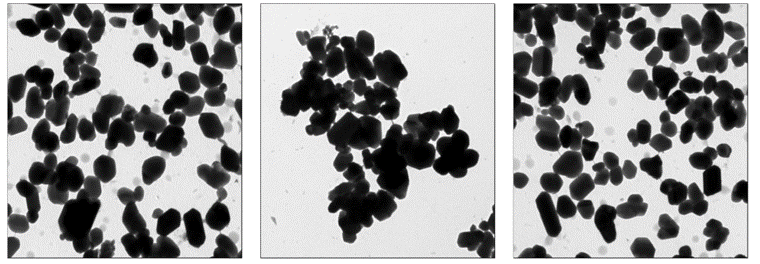
\includegraphics[width=\linewidth]{real_data.png}
  \caption{Real data.}
  \label{fig:real_data}
\end{figure}
This work focuses on segmentation of convex objects. The work will continue earlier research where a framework to segment (estimate contours) of partially overlapping nanoparticles was developed~\cite{zafari2017comparison}. The framework consists of three steps: 
1) detection of concave edge points, 
2) grouping of the resulting edge segments to form contour evidence, and 3) estimating the full contours of the objects (see Fig.~\ref{fig:concave_framework})~\cite{Zafari15,zafari-bb}.

\begin{figure}[ht]
  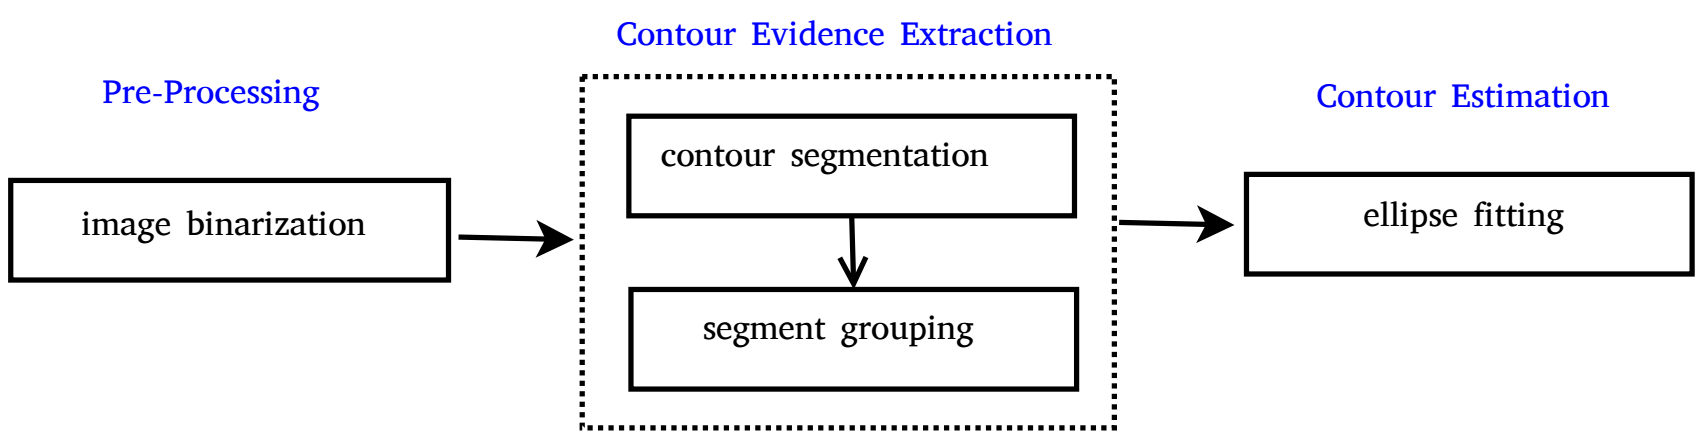
\includegraphics[width=\linewidth]{concave-framework.png}
  \caption{Concave points based framework.~\cite{zafari-bb}}
  \label{fig:concave_framework}
\end{figure}

In order to be able to estimate the full contour the object with partially observed edges, all the edge points or edge segments belonging to the same object need to be grouped. To do this shape analysis of the resulting object is needed. This can be done by employing a grouping method that defines how likely two edge segments belong to the same object, that is how well the resulting object fits the prior information about the object shapes or contour model. 


\subsection{Objectives and delimitations}
\label{sec:objectives}


 The aim of this Master’s thesis is to develop an efficient grouping strategy that group the contour segment which belongs to the same object.


The objectives are as follows:
\begin{enumerate}
\item find and develop different grouping methods using the contour model/shape criteria/metrics (e.g. convexity) for objects;
\item evaluate the grouping methods using the existing framework;
\item perform parameter optimization and parameter sensitivity analysis for the developed method.
\end{enumerate}



\subsection{Structure of the thesis}

In the rest of thesis has the following structure. Chapter 2 gives a brief overview of existed contour segmentation methods. This Chapter contains a description of seed point extraction methods, concave point-based method, and edge segment grouping methods. Chapter 3 presents the new proposal. Chapter 4 contains the information about experiments and validation of the methods. Chapter 5 discusses the findings and describe goals of the further research. Chapter 6 concludes the thesis and give a brief overview of the task, the solution, and the results.

% ---------------------------------------
%             RELATED WORK
% ---------------------------------------

\section{SEGMENTATION OF OVERLAPPING CONVEX OBJECTS}
\label{sec:related}
There are two typical approaches to solve the segmentation of overlapping convex object segmentation problem. The first is based on the extraction of seed points~\cite{zafari-thesis}, special points, that are geometrical centers of overlapping objects. The second approach is based on concave point detection~\cite{Zafari15}. This method extracts visible boundaries of overlapping objects and detects the special concave points, that are corners between overlapping objects.  

\subsection{Seed point-based methods}
A typical framework for segmentation of overlapping object usually consists of next specific steps~\cite{zafari-thesis}:


\begin{enumerate}
\item Seed region/point extraction. In this step, there is extracting points or regions of each overlapping object. The seed points usually refer to a geometrical center point of anticipated overlapping objects. The goal of this step is to recognize the number of the individual overlapping objects. The count and position of the detected points in this step are not the final and can be improved during next steps.
\item Contour evidence extraction. The goal of this step is the determination of the counter-evidence, the visible parts of the object boundaries, that are used to determinate the hide parts of overlapped objects. The aim of this step to group edge points that belong to each object using information about seed points or seed region from the previous step.
\item Contour estimation. During this step, the full contour of all overlapping objects is estimated based on results of previous steps.
\end{enumerate}


The schema of the algorithm is shown in Figure~\ref{fig:general_framework}.

\begin{figure}[ht]
  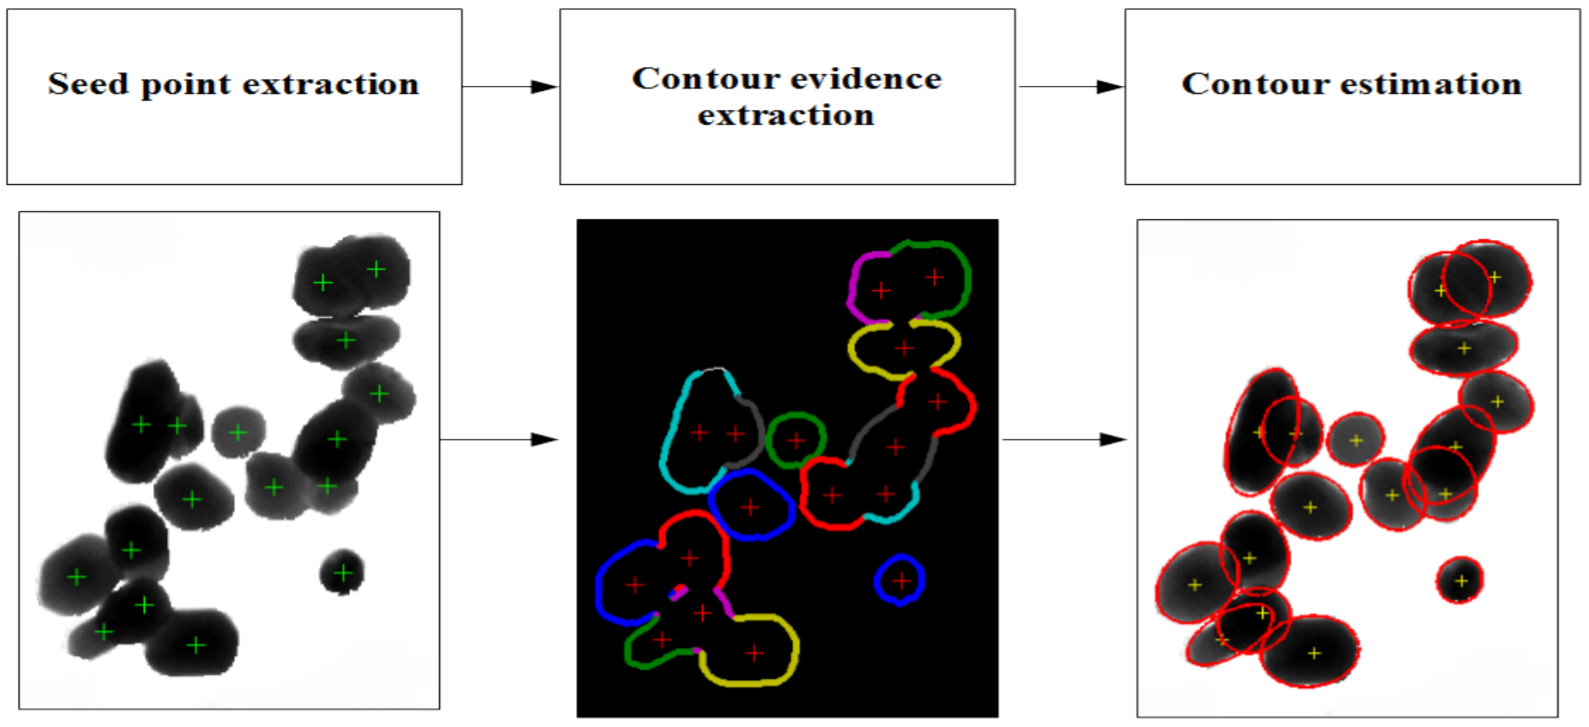
\includegraphics[width=\linewidth]{General_framework.png}
  \caption{Framework based on seed points.~\cite{zafari-thesis}}
  \label{fig:general_framework}
\end{figure}

The seed point extraction one of the most important steps in overlapping object segmentation. It has a big impact on the accuracy of the final segmentation result. Seed point extraction produces a priori information that uses in counter evidence extraction and contour estimation. The goal of this step is to recognize the number of the individual overlapping objects in the image and correspond them with seed points. The description of the methods is based on~\cite{zafari-thesis}.

\subsubsection{Local Convergence Filters}
The description of the local coverage filters is based on paper~\cite{LCF}.
This group of filters is one of the most used algorithms to detect seed points. Local Convergence Filters (LCF)~\cite{LCF} is based on evaluating the degree of convergence of the gradient
vectors within a local area (support region) toward a pixel of
interest. This method does not use the gradient magnitude that makes LCF tolerant to illumination variation effects.
These filters share the same
definition for the convergence degree but differ from their approach in defining the support
regions. The examples of such filters are coin filter~\cite{LCF_CF}, IRIS filter~\cite{LCF_CF}, adaptive ring filter~\cite{LCF-ARF}, sliding band filter~\cite{LCF-SBF}. They are shown in Figure~\ref{fig:LCF-alg}.

\begin{figure}[ht]
  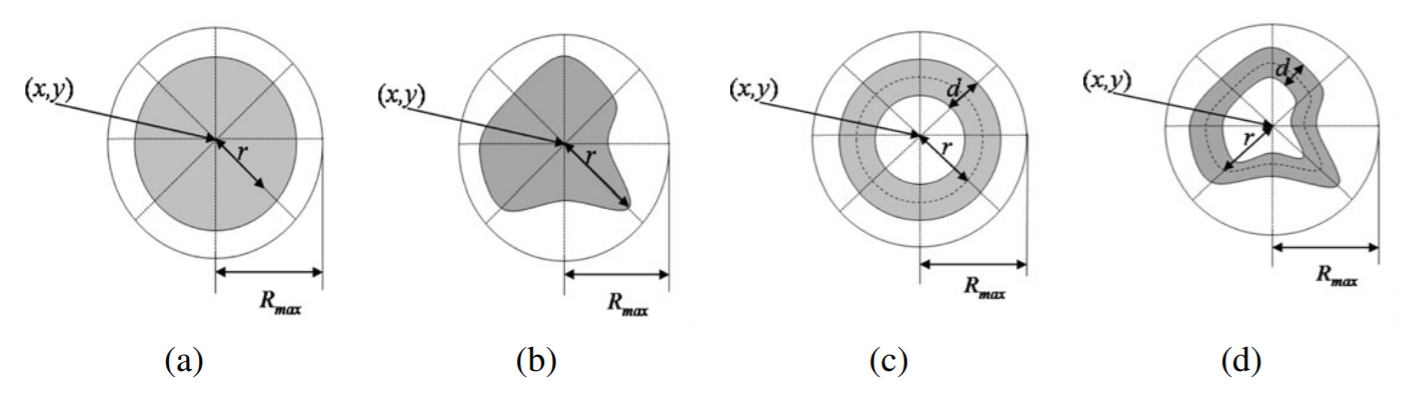
\includegraphics[width=\linewidth]{LCF.png}
  \caption{LCF filters: (a) Coin filter; (b) IRIS filter; (c) Adaptive ring filter; (d) Slide band filter.~\cite{LCF}}
  \label{fig:LCF-alg}
\end{figure}


CF or the Convergence Index Filter~\cite{LCF_CF} is the basic LCF method. The support region in this method has a circular shape. The value of the radius is varied in search for the one which
corresponds to maximum convergence, limited by a maximum
radius. 

The IRIS filter (IF)~\cite{LCF_CF} is an modification of the CF filter. The differs from the previous one in that the radius of a support region for every direction changing independently,. As a result, this filter is not restricted to circular shapes and can handle more complex objects. 


The Adaptive ring filter (ARF)~\cite{LCF-ARF} define a ring-shaped convergence region. The motivation for this support
region is the idea that the convergence of a convex
object is mostly originated at those objects’ edges, which makes the method more noise-resistant.


The Sliding Band Filter (SBF)~\cite{LCF-SBF} unites both limited band search of the ARF and the shape flexibility of the IF. 
The result of work of SBF looks like the result of IRIS but provides better separating of overlapping objects.


LCF methods have one common shortcoming. These methods are based just on gradient orientation and ignore gradient magnitude, that can lead to big segmentation errors when gradient magnitude
is low~\cite{LCF}. 



\subsubsection{Ultimate Erosion for Convex Sets}

Ultimate Erosion for Convex Sets (UECS)~\cite{UECS} is an iterative morphological algorithm that extracts
the seed regions from overlapping object. UECS is an extension of the Ultimate Erosion
(UE) method with a modified stopping criteria~\cite{UECS}. The algorithms consist of two stages. On the first stage, the image is decomposed into disjoint convex sets. This stage is based on the Ultimate Erosion algorithm with medicated stooping criteria that make possible to avoid over-segmentation. The result of this stage is set of disconnected objects. In the second stage, the input segments transform by the Gaussian mixture model on B-splines to fully connected particles. The algorithm has one key parameter, the threshold for concavity measurement~~\cite{zafari-thesis}. This parameter depends on data and should be estimated manually. 
The detailed visualization of the steps of the algorithm is shown in Figure \ref{fig:UECS-alg}.

\begin{figure} [ht]
  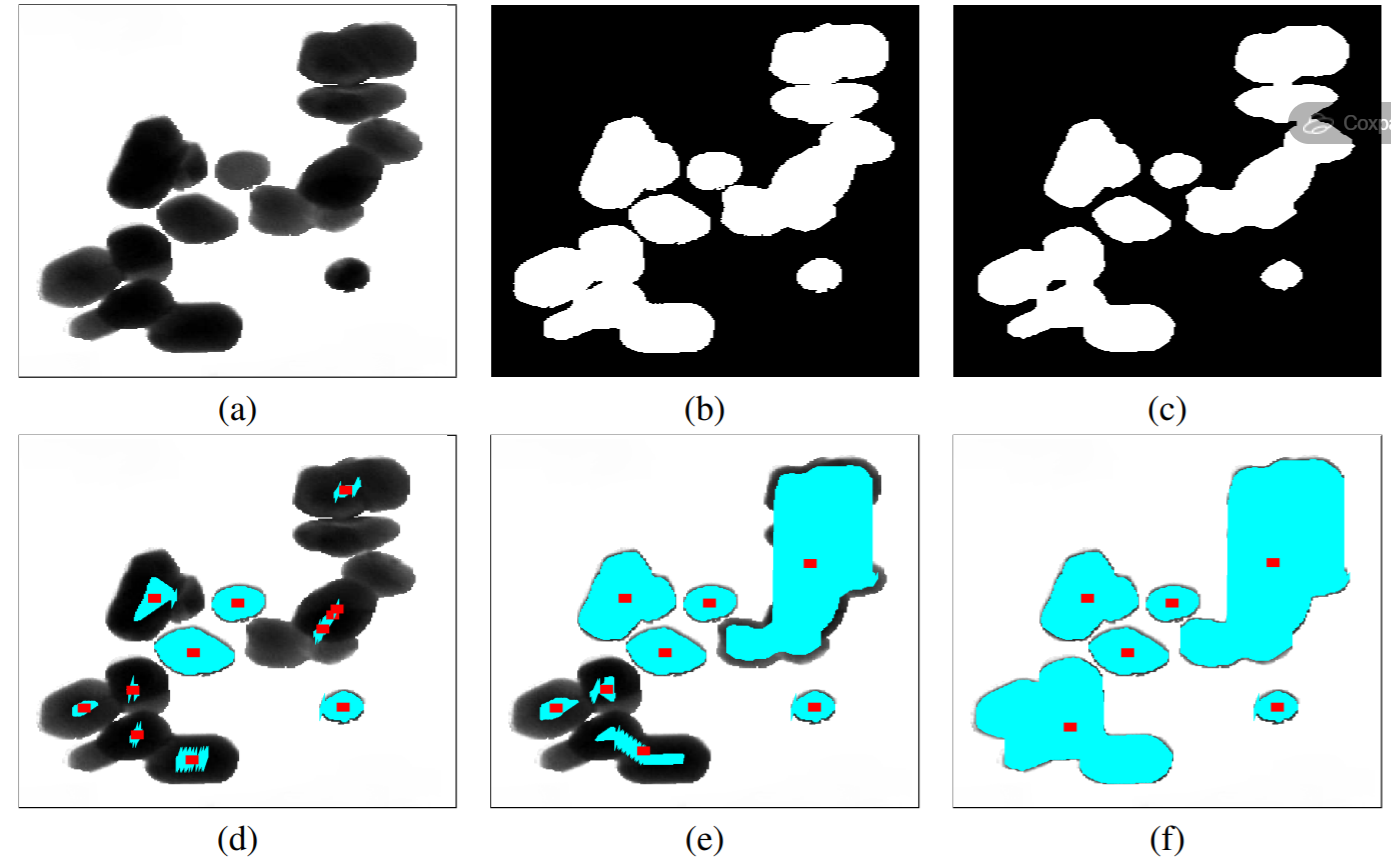
\includegraphics[width=\linewidth]{UECS.png}
  \caption{UECS seed point extraction: (a) Original image; 
    (b)Binary image; 
    (c) Binary image after morphological opening; 
    (d) Seed points identified with threshold 0.1;
    (e) Seed points identified with threshold 0.2;
    (f) Seed points identified with threshold 0.3.~\cite{zafari-thesis}}
  \label{fig:UECS-alg}
\end{figure}

\subsubsection{Distance Transform}

The Distance Transform (DT)~\cite{DT} is a simple operator that is usually applied to image segmentation~\cite{zafari-thesis}. The DT transform each pixel in its small region of the interest.
The method is visualized in Figure~\ref{fig:DT_img}. The algorithm~\ref{alg:DT} shows the main steps of the method.

\begin{algorithm} [H]
   \begin{enumerate}
        \item binarization of the image;
        \item morphological opening of the image;
        \item interactively mapping of the value each pixel to the minimum value of the pixel area by DT;
        \item the seed point and region estimation by the predefined threshold.
    \end{enumerate}
    \caption{Distance Transform filter~\cite{DT-bactery}.}\label{alg:DT}
\end{algorithm}

\begin{figure} [ht]
  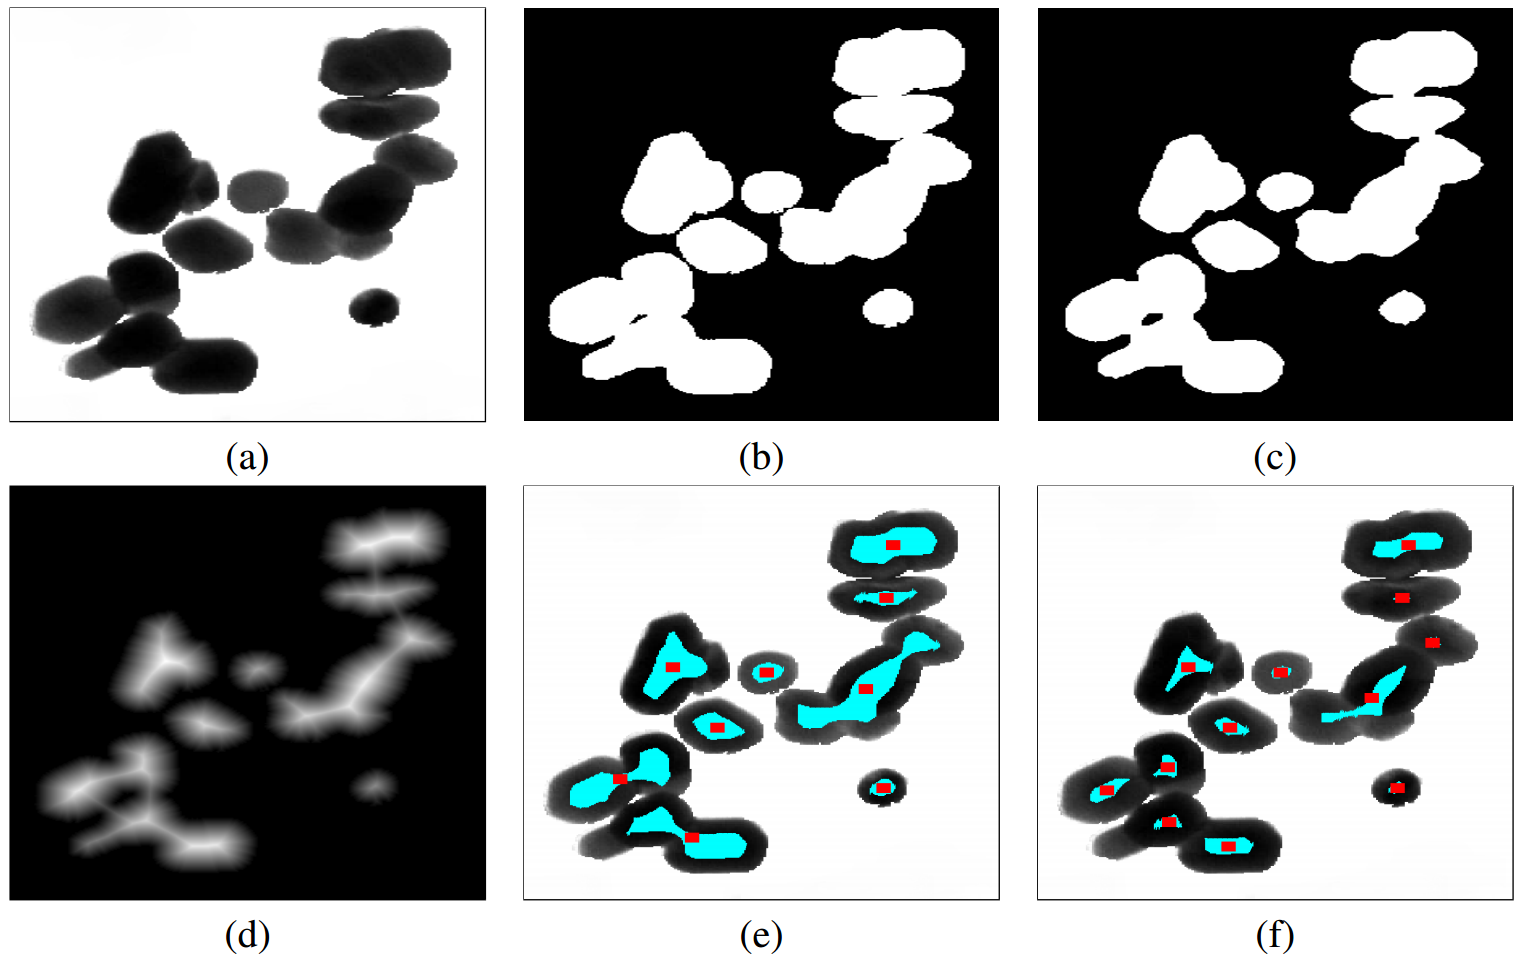
\includegraphics[width=\linewidth]{DT.png}
  \caption{
    Distance Transform seed point extraction: (a) Original image; (b) Binary image;
    (c) Binary image after morphological opening; 
    (d) Result of DT; 
    (e) S Seed points identified with threshold 0.6; 
    (f)  Seed points identified with threshold 0.7~\cite{zafari-thesis}.}
  \label{fig:DT_img}
\end{figure}


\subsubsection{BE-FRS}
The current state-of-art technique in seed point extraction of elliptical objects is Bounded Erosion Fast
Radial Symmetry method (BE-FRS)~\cite{BE-FRS}. This technique uses two common properties of elliptical objects: convexity and symmetry.
It uses a hybrid model consisting of morphological erosion and the FRS in a
silhouette image to obtain the seed points of each object, while each seed point
is used to mark an individual object. In particular, it makes each edge point vote
in the gradient direction according to the current distance $d \in R$. The center
of gravity of each vote region is taken as its seed point, which is used to mark
each object in the image. 

The applying Bounded Erosion~\cite{BE} before FRS improves the quality of seed point extraction by smoothing the shapes of overlapped objects.

Fast radial symmetry (FRS)~\cite{FRS}  is a wide-used method that transforms the original
image to a new representation, highlighting the local radial symmetry of the image gradient.
The main idea pf FRS that  every edge pixel in the image giving a vote for the plausible radial symmetry at some specific distance from that point. This step relies on two parameters $R$ and $T$ , $R = [R_{min} , R_{max}]$ which represents the range of the vote of each point, while $T$ indicates the threshold for the distance between two adjacent seed points. 

\subsection{Concave point-based methods}
Another approach for segmentation of overlapping objects is the concave point-based method. That method was well-described in~\cite{compare-cpd}. The idea of this methods is dividing the contour of the group of overlapping objects to set of segments separated by special points, so-called concave points. The main steps of the methods are shown in Algorithm~\ref{alg:CPD}. The visualization of the method is shown in Figure~\ref{fig:Contour-segmentation}.

\begin{algorithm} [H]
    \begin{enumerate}
        \item Image binarization;
        \item Dividing the image into the separate Regions of Interest (ROI), that contains particles or groups of overlapping particles.
        \item Extraction of the contour of the whole ROI;
        \item Splitting the contour to the edges and extracting the concave points;
        \item Grouping of segments that are parts of one particle;
        \item Ellipse fitting;
    \end{enumerate}
    \caption{Concave point-based method~\cite{Saddik}.}\label{alg:CPD}
\end{algorithm}

\begin{figure} [ht]
  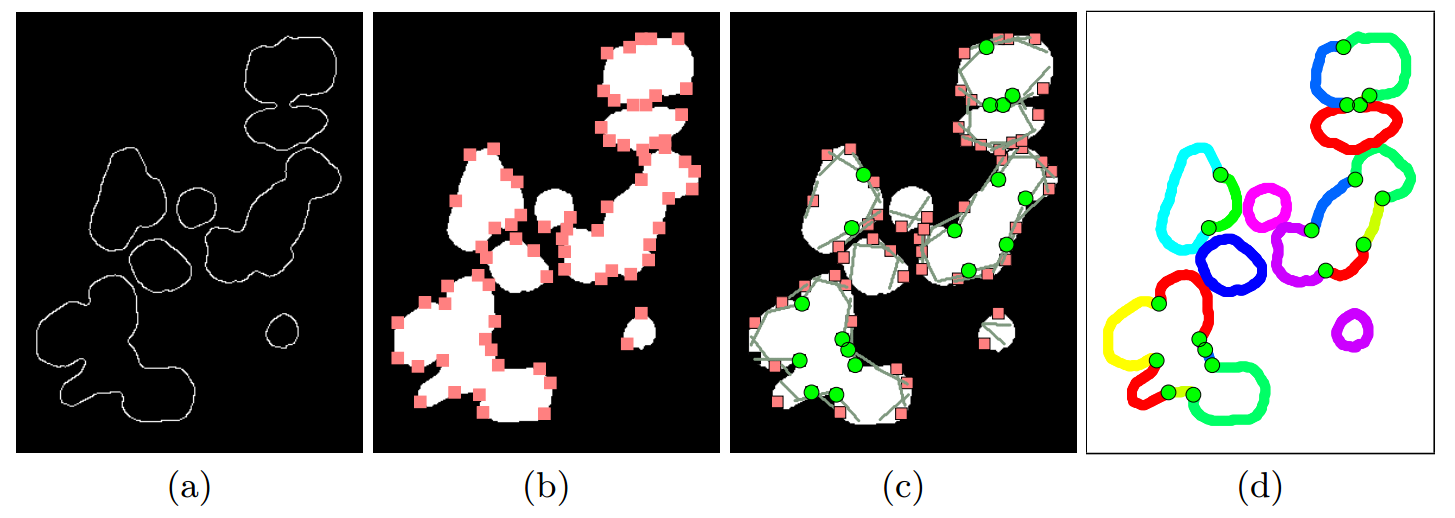
\includegraphics[width=\linewidth]{concave_points.png}
  \caption{: Contour segmentation: 
    (a) Counter map; 
    (b) Corner detection; 
    (c) Concavity points extraction;
    (d) Contour segmentation.~\cite{Zafari15}}
  \label{fig:Contour-segmentation}
\end{figure}




\subsubsection{Edge segmentation}
Image binarization can be performed by Otsu algorithm~\cite{otsu}. Separating the image into regions of interest is simple and well-described in~\cite{ROI}.
There are follows methods that performs the segments detection~\cite{compare-cpd}:
\begin{enumerate}
    \item \textit{Curvature based methods}. These methods are based on computation of curvature values of every edge points $c_i = (x_i,y_i)$ by the following formula:
        \begin{equation}
            k = (x_i'y_i''-y_i'x_i'') / (x_i'^2+y_i'^2)^{3/2}.
        \end{equation}
        Furthermore, methods select special dominant points, which are local extrema for $k$ value. There are different strategies of pick over concave points from the set of dominant points. A method purposed by Wen \emph{et al.}~\cite{curv-wen}  select points by a preset threshold, Zafari \emph{et al.}~\cite{Zafari15} approach is based choosing points that neighbours do not reside inside the object, Dai \emph{et al.}~\cite{curv-dai} presents a method that calculates the triangle area of a point with neighbour and if it is positive marks the point as concave.
    \item \textit{Skeleton methods}. This group of methods uses the skeleton and boundary information. The idea of method purposed by Samma\emph{et al.}~\cite{bnd-skeleton} is the identification of concave points by computing the intersection between skeleton and contour points. The method purposed by Wang \emph{et al.}~\cite{skeleton} detects concave points if the shortest distance to skeletons is more than a preset threshold.
    \item \textit{Chord methods}. The main idea of these methods is the identification of concave points as points that have the maximum distance to the concave area chord. There are several methods to estimate concave point area which are described in 
    ~\cite{chord-farhan,chord-kumar}.
    \item \textit{Polygon methods}. These groups of methods are a well known way to represent the contour of the element as a sequence of dominant points. A dominant point is a point $c_i$  of the contour that is not placed on the line which between $c_{i-1}$ and $c_{i+1}$. A dominant point $c_i$ is a concave point if the line $c_{i-1}c_{i+1}$ does not pass throw inside the object and the angle between the lines $c_{i-1}c_{i}$ and $c_{i}c_{i+1}$ is in the range of predefined thresholds in~\cite{Bai20092434} . Zhang  \emph{et al.}~\cite{bubble} define a dominant point as a concave if ${c_{d,i-1}c_{d,i}}\times {c_{d,i}c_{d,i+1}}$ is positive. Sahar \emph{et al.}~\cite{compare-cpd} unites two methods~\cite{bubble} and~\cite{Bai20092434} to avoid any predefined parameters of the concave point detector.
\end{enumerate}
\subsubsection{Segment grouping}
The next step is grouping such segments which belong to one object, see Figure~\ref{fig:Segment-grouping}. Zhang~\cite{bubble} purposed an average distance deviation criterion (ADD) as a metric for segment grouping. ADD is based on a heuristic that all particles have elliptical shapes. Segment $s_i$ will be grouped with $s_j$ if the goodness of ellipse fitting merged segments is higher than the goodness of separate ellipse fitting.

\begin{figure} [ht]
  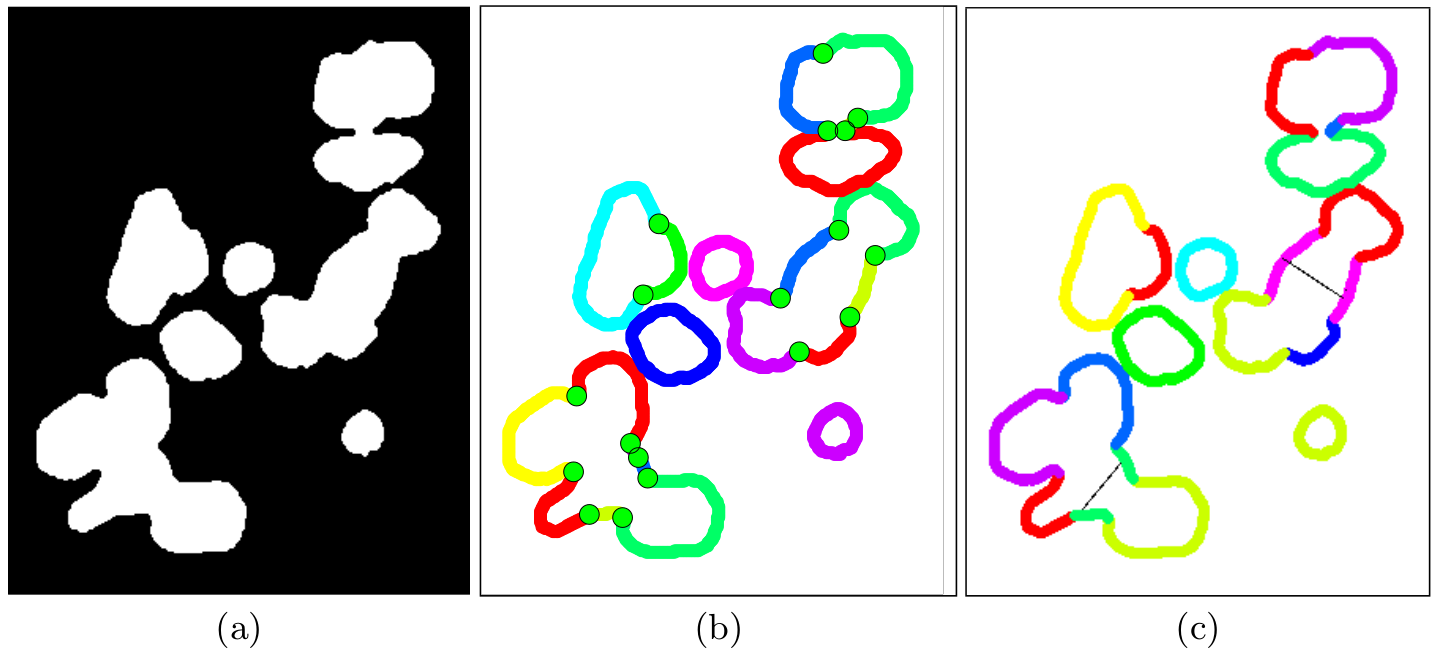
\includegraphics[width=\linewidth, scale=0.5]{segment-grouping.png}
  \caption{: Contour segmentation: 
    Segment grouping: 
    (a) Original image; 
    (b) Contour segmentation;
    (c) Segment grouping.~\cite{Zafari15}}
  \label{fig:Segment-grouping}
\end{figure}

The naive edge segment grouping algorithm iterates over each pair of contour segment, checking if they can be united in one ellipse. However, combinations of $n$ edges into $p$ is very complicated task according to the Stirling number formula:
    \begin{equation}
        P(n,p) = \frac{1}{p!}\sum_{n_1+n_2+...+n_p=n}\frac{n!}{n_1!...n_p!}.
    \end{equation}
To deal with the problem of a big amount of permutation researchers use some heuristics. Langlard \emph{et al.}~\cite{LANGLARD2018} purposed the method that divides the cluster of overlapped elliptical objects to several sub-clusters. To do this, the authors search special split lines with the algorithm that was purposed by Farhan \emph{et al.}~\cite{farhan}. The visualization of the method is shown in Figure~\ref{fig:cluster-decomposition}.



\begin{figure}[htp]
    \centering {
        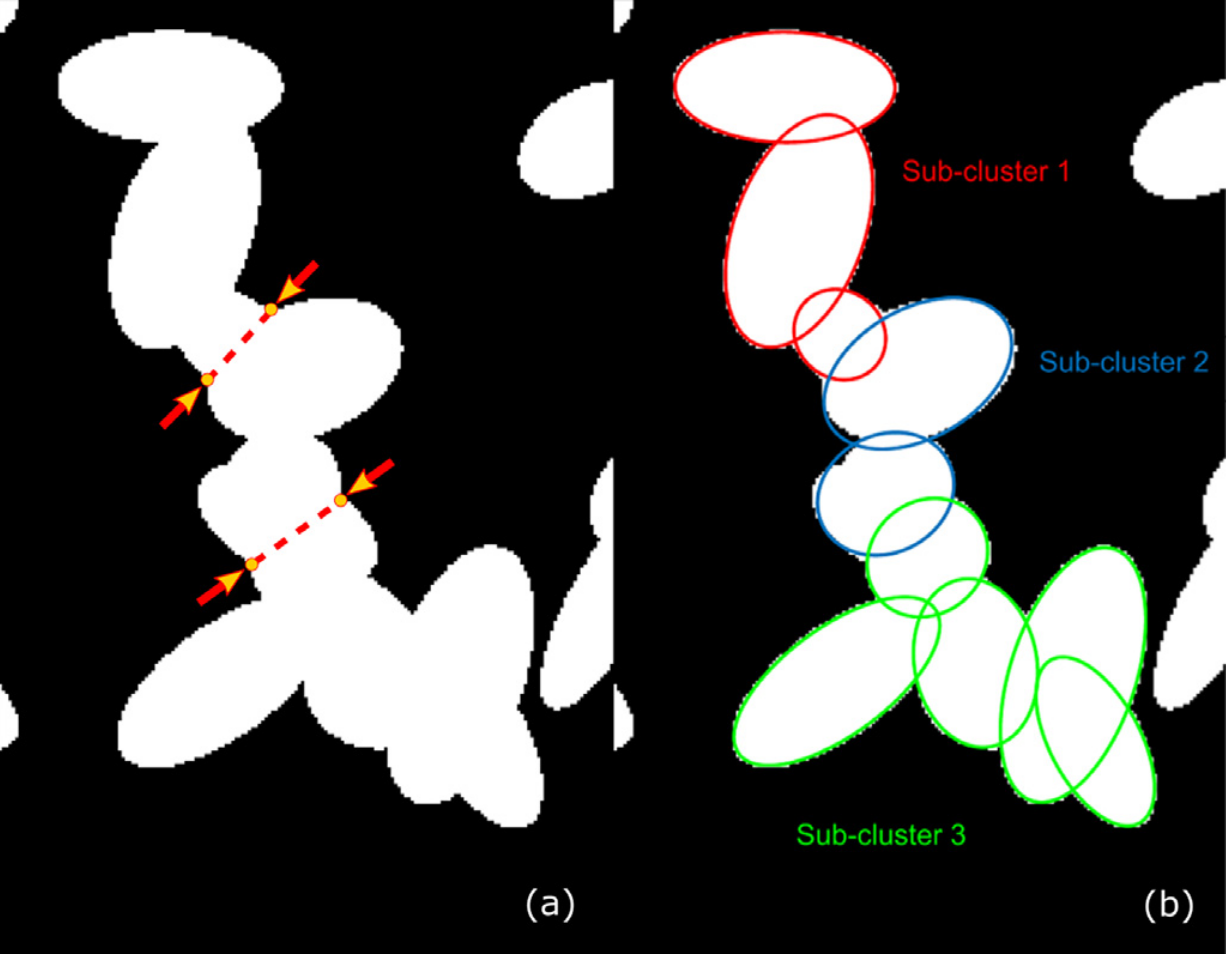
\includegraphics[width=100mm, scale=0.5]{subgrouping.png}
        \caption{Illustration of cluster decomposition and ellipse fitting: (a) Initial cluster and detected split (b) resulting sub-clusters and ellipse fitting.~\cite{LANGLARD2018}.}
        \label{fig:cluster-decomposition}
    }
\end{figure}

Zafari \emph{et al.} proposed two methods for segment grouping.  The first method that described in~\cite{zafari-bb} limits search space by a rule that distance between centers of segments is less than a predefined threshold value. The second method~\cite{zafari-bb} is based on the branch and bound optimization algorithm. The authors presented a new cost function that uses some properties of elliptical objects like ellipticity, convexity, and symmetry. 



\subsection{Contour Estimation}

The last step in the segmentation of overlapped object process is contour estimation. The most uses method for contour estimation is an Ellipse fitting method. This method can be applied to many tasks in a segmentation of overlapped object area ~\cite{BE-FRS,Zhao2017,zafari-bb,LANGLARD2018}. This method uses the assumption that overlapped objects have an elliptical form. The Ellipse fitting approach is based on minimization the sum of distances between points and an ellipse. The definition of ellipse equation is:
\begin{align}
    F(\textbf{a},(x,y)) &= a_0x^2 + a_1xy + a_2y^2 + a_3y + a_4y + a_5 = \textbf{a}^T \mathbf{x} = 0,
\end{align}
where $x$ and $y$ are the input points. The authors of fundamental researches~\cite{acos_1} formulate the problem as a direct minimization of the equation $E = \sum_{i=1}^{n}d^2(\textbf{a}),$
where $d(\textbf{a}) = \sum_{i=1}^N{F(x_i, y_i)}$. The result of algorithm work is show in Figure~\ref{fig:ellipse-fitting}.

\begin{figure}[htp]
    \centering {
        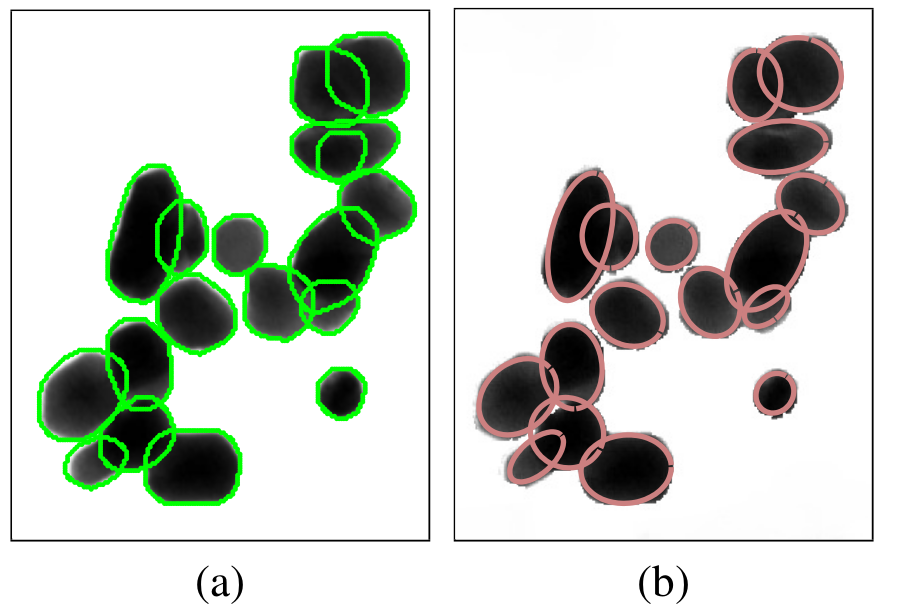
\includegraphics[width=\linewidth]{ellipse_fitting.png}
        \caption{Ellipse fitting method: (a) Ground truth fitting (b) Ellipse fitting.~\cite{BE-FRS}.}
        \label{fig:ellipse-fitting}
    }
\end{figure}


\section{PROPOSED METHODS}
\label{sec:proposed}

This section contains a description of a proposed method for segmentation of convex overlapped objects.
The segmentation method is based on concave points extraction method and has the next pipeline: 

\begin{enumerate}
    \item Image binarization and edge extraction;
    \item Concave points detection and segmentation;
    \item Segment grouping.
\end{enumerate}

The novelty of the proposed method is in segment grouping stage. However, the other stages are very important for right grouping, so there is a brief explanation of all stages.


\subsection{Image binarization and edge extraction}

This stage is the most simple but very important part of the segmentation process. It consists of following steps: image binarization, smoothing the binary image, and edge extraction.

\begin{enumerate}
    \item Binarization of original gray-scale image by Otsu method~\cite{otsu}. This algorithm is a state-of-art algorithm that divides the image into two classes by adaptive threshold. It uses the histogram of the image for threshold searching process. It maximizes "between class variance" of the segmented classes. Otsu proves that Minimizing "within class variance" is same as maximizing "between class variance" of the segmented classes. And maximizing "between class variance" is computationally less expensive than minimizing "within class variance".
    \item Smoothing and eroding the binary image. Usually, the original images contain some noise and sharp boundaries, that must be smoothed. To deal with it proposed framework uses morphological erosion~\cite{UECS} with 3-pixel disk structuring element. It smooths the boundaries and reduces a noise that can be detected as small particles.
    \item Edge extraction by Canny detector~\cite{Canny}. The Canny operator works in a multistage process. First of all the image is smoothed by Gaussian convolution. Then a simple 2-D first derivative operator (somewhat like the Roberts Cross) is applied to the smoothed image to highlight regions of the image with high first spatial derivatives. Edges give rise to ridges in the gradient magnitude image. The algorithm then tracks along the top of these ridges and sets to zero all pixels that are not actually on the ridge top so as to give a thin line in the output, a process known as non-maximal suppression. The tracking process exhibits hysteresis controlled by two thresholds: $T1$ and $T2$, with $T1 > T2$. Tracking can only begin at a point on a ridge higher than $T1$. Tracking then continues in both directions out from that point until the height of the ridge falls below $T2$. This hysteresis helps to ensure that noisy edges are not broken up into multiple edge fragments.
\end{enumerate}

\subsection{Concave points detection and segmentation}

For concave point extraction was selected algorithm proposed by X.C. He in~\cite{CSS}. The algorithm was selected because it has some key features.  The detector first uses an adaptive local curvature threshold an not the global threshold parameter. Second, the angles of corner candidates are checked in a dynamic region of support that reduces the number of false predicted concave points.

Concave point extraction can produce too many concave points in one small area, especially, in hard cases like an intersection of many objects. The framework uses next filter algorithm, if the distance between concave points is less then some threshold, the points will unite to one point between them (~\ref{fig:concavepoints})

\begin{figure}[htp]
    \centering {
        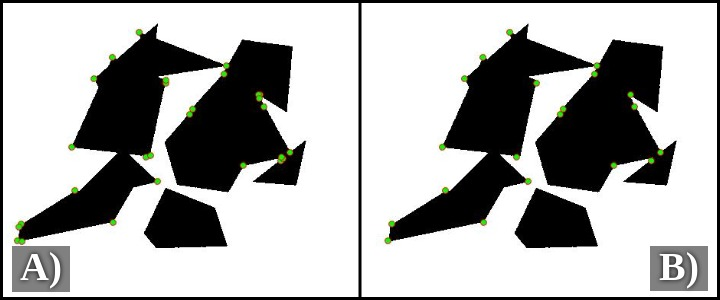
\includegraphics[width=\linewidth]{pjimage.jpg}
        \caption{Concave points extraction: a) before reducing, b) after reducing.}
        \label{fig:concavepoints}
    }
\end{figure}
After detecting concave points they are projected into edges and divided them into segments, that are bounded by concave points.

\subsection{Segment grouping}

In this stage, the framework unites segments to one group that belong to one concave object. It consists of two main parts: preprocessing and branch and boundaries algorithm.

\subsubsection{Preprocessing} 
During this step, the framework creates so-called \textbf{\textit{grouping matrix}}, a special concavity matrix of all segments, that contains 'true' if two segments can be, hypothetically, united to one group, and 'false' if not. To determine the result for two segments are used two heuristics: adjacency and attainability.

\textit{Adjacency} - is a simple heuristic that based on an idea that two neighbor segment cannot be grouped, because in another way there could not be a concave point between them  (see Image~\ref{fig:heuristics}(a). 
\textit{Attainability} is more complicated heuristic which validates that two segments can be united to one polygon, and this polygon does not intersect other segments (see Image~\ref{fig:heuristics}(b).


\begin{figure}[htp]
    \centering {
        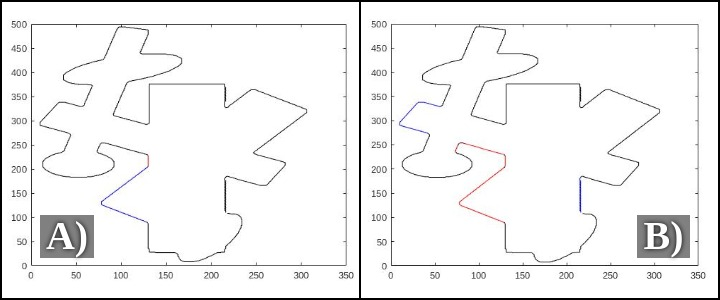
\includegraphics[width=\linewidth]{heuristics.jpg}
        \caption{Examples of restricted pairs of segment: a) neighbours, b) a pair that intersects other segments.}
        \label{fig:heuristics}
    }
\end{figure}

\subsubsection{Branch and boundaries}
The segment grouping task can be represented as a combination problem of optimal separation of N objects to M groups by some criteria. However, it is an NP-hard problem and cannot be solved by brute force algorithms. One of the best and simple methods to solve NP-hard problems is Branch and Boundaries algorithm.  BB is efficient for optimization problem since it avoids exhaustive enumeration using the value of the current optimal solution
and defining bounds for the function to be optimized. 

Firstly, the algorithm creates initial root node with an empty group. Next, the algorithm interactively tries to add new child nodes that extending parent groups with new segments. If the grouping criteria of a child node are bigger then parent node, the algorithm removes that node and do not evaluate parents node for it. That algorithm is well-described in~\cite{zafari-bb}.  The groping process of Branch and Boundaries algorithm is shown in Picture~\ref{fig:bb}.

\begin{figure}[htp]
    \centering {
        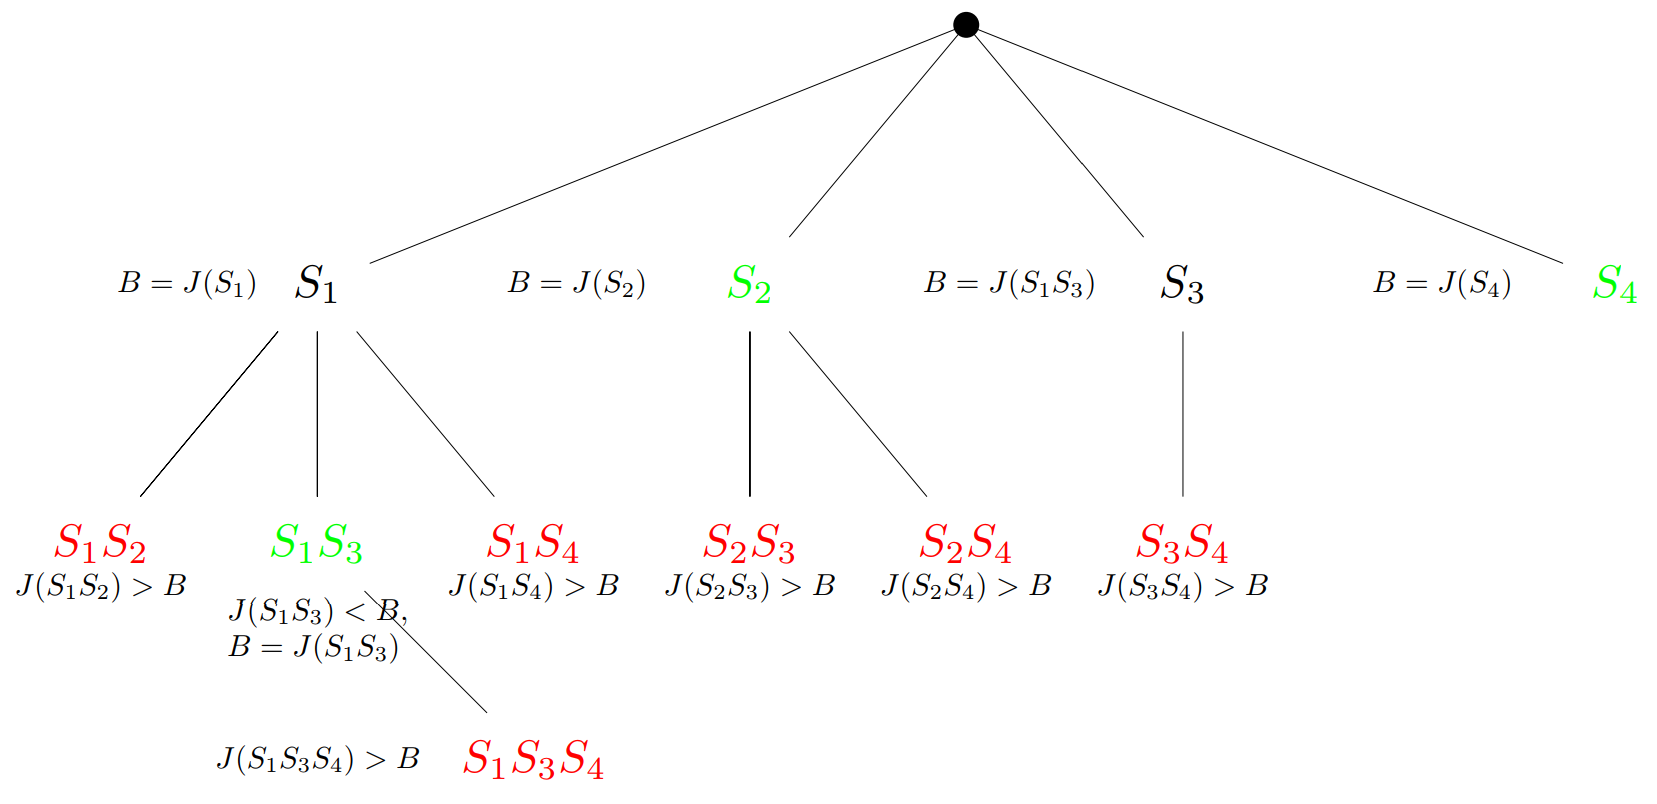
\includegraphics[width=\linewidth]{bb.png}
        \caption{Example of Branch and Boundaries groups tree~\cite{zafari-bb}.}
        \label{fig:bb}
    }
\end{figure}

\subsubsection{Grouping criteria}

The key part of BB algorithm is grouping criteria or cost function. This criteria represent the "quality" of grouping and allow the algorithm to compare two segment groups. To estimate the grouping criteria researcher believe that particles have an elliptical form and create cost function based on symmetry, convexity and ellipticity~\cite{zafari-bb}.

For this framework was developed another cost function that based on a hypothesis that object has a convex form and are similar to one of the next type of shapes: ellipse, quadrilateral, triangle. The grouping cost calculation algorithm consists of several parts and pseudo-code of it is shown in Algorithm~\ref{alg:CostFunction}.

\begin{enumerate}
    \item The segments in a group must be adjacent to each other in grouping matrix. If at least one pair of segments is not adjacent, the grouping cost will be infinity.
    \item  Reordering of segments. It is a necessary operation because the convexity checking function requires segments sorting by clockwise order. The idea of sorting algorithm is following. Each segment from input array must be added to the result array greedy by maximization the total area of a polygon based on result vector. The complexity of the algorithm is $O(n^2)$.
    \item Shape fitting. For this framework, the type of figures was limited by ellipse, quadrilateral, and triangle, as the most common types. To determinate the similarity of a segment group to one to the shape are used the following trick. The framework calculates the area of the segment group polygon. Next, the algorithm represents the segments as a cloud of points and build around it the ellipse, quadrilateral, and triangle with minimal area. The similarity of the group is calculated by the next formula: 
    \begin{equation}
        similarity = \frac{min(S_{convexTriangle},S_{convexEllipse},S_{convexQuadrilateral})}{S_{segments}}
        \label{eq:simularity cost}
    \end{equation}
    \item Groping cost calculation.  The grouping criteria should encourage the big amount of segment in a group. It can be done very simple by dividing the result of previous steps by the count of segments. So the final grouping criteria are:
    \begin{equation}
        J = \frac{similarity}{size(segments)}
    \label{eq:fullCost}
    \end{equation}
\end{enumerate}


\begin{algorithm} [H]
    \SetAlgoLined
    \KwData{segments, groupingMatrix}
    \KwResult{cost}
    \If {one or more pair of segment is not adjacent in grouping matrix} {
     \Return {$\infty$ }
    }
    sort segments clockwise\;
    check segments group convexity\;
    \If {group is not convex} {
        \Return {$\infty$ }
    }
    calculate simularity by equation~\ref{eq:simularity cost}\;
    calculate grouping cost by equation~\ref{eq:fullCost}\;
    \Return{grouping cost}
\caption{Cost function.}\label{alg:CostFunction}
\end{algorithm}

\section{EXPERIMENTS}
\label{sec:experiments}

\subsection{Data}
For validation of developed framework was used two types of data: real data and synthetic data.
 
The synthetic dataset (see figure~\ref{fig:data}-A) consists of images with overlapping
objects of different types, as ellipses, triangles, and quadrilateral. All objects uniformly randomly translated, scaled and rotated. All generated images have size 400x500 pixels and maximum rate of overlapping area 40\%. There were 40 generated images. Every image was generated with additional information about the shape of figures.

The real dataset contains images of nanoparticles, captured
using transmission electron microscopy (see figure~\ref{fig:data}-B). In result, the dataset includes 11 images of 4008x2672 pixels. Approximately 200 particles were marked manually in each picture by a specialist. The explanations consist of manually drawn contours of the objects. 

\begin{figure}[htp]
    \centering {
        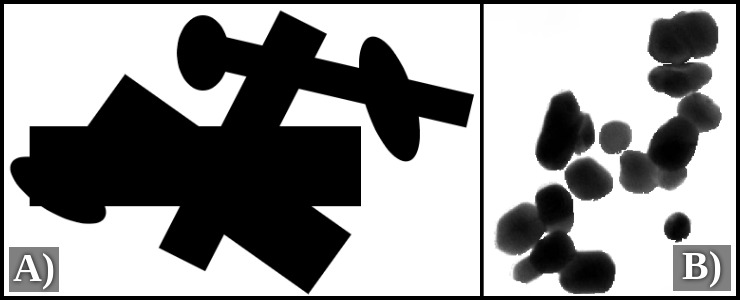
\includegraphics[width=\linewidth]{data2.jpg}
        \caption{Example of data images: (a) Synthetic data (b) Real data.}
        \label{fig:data}
    }
\end{figure}

\subsection{Evaluation criteria}
Segment grouping task can be evaluated, as clusterization problem, where the count of predicted classes may differ from ground truth. One of the best metrics of clusterization id Maximum-Match-Measure~\cite{mm-estimate}. For the evaluating criteria were selected next metric. This measure tries to find an optimal matching between the predicted results and the true classes.

For instance, there is 4 predicted groups and 3 ground truth groups. The matrix of similarity looks like:
\begin{equation}
similarity = 
        \begin{bmatrix}
            2& 7 & 3 \\
            6& 2 & 3\\
            3& 3& 1\\
            2& 1 & 8
        \end{bmatrix}
    \end{equation}
Which can be read like this: predicted group 1 has 2 elements from expected group 1, 7 from expected group 2 and 3 from expected group 3, and so on.
Maximum-match tries to find the 3x3 matrix with maximum trace (diagonal sum). In this case, it'd be

\begin{equation}
MMmatrix = 
        \begin{bmatrix}
            6& 2 & 3\\
            2& 7 & 3 \\
            2& 1 & 8
        \end{bmatrix}
    \end{equation}
The result for this case will be $mm = \frac{6+7+8}{41}$.

\subsection{Results}

The proposed method was compared with two methods: Branch and Boundaries algorithm based on concave points~\cite{zafari-bb} and the algorithm based on seed points~\cite{Zafari15}. The result for synthetic and  real data was shown in Table~\ref{tab:syndata} and Table~\ref{tab:realdata} respectively.


\begin{table}[hpt]
\begin{center}
\caption{The result of validation comparing for synthetic data.\label{tab:syndata}}
\begin{tabular}{ |p{2cm}||p{3cm}|p{3cm}|p{4cm}|  }
 \hline
 Number & Proposed method & Zafari BB~\cite{zafari-bb} &Zafari Seed point~\cite{Zafari15}\\
 \hline
 1   &  0.73&  0.54& 0.43\\
 2   &  0.68&  0.46& 0.45\\
 3   &  0.53&  0.23& 0.21\\
 4   &  0.88&  0.45& 0.33\\
 5   &  0.91&  0.51& 0.45\\
 6   &  0.44&  0.34& 0.31\\
 7   &  0.79&  0.47& 0.56\\
 8   &  0.85&  0.72& 0.66\\
 9   &  0.47&  0.44& 0.47\\
 10   &  0.91&  0.53& 0.35\\
 11  &  0.72&  0.23& 0.25\\
 12   &  0.73&  0.50& 0.45\\
 13   &  0.86&  0.34& 0.34\\
 14   &  0.69&  0.21& 0.39\\
 \hline
 \textbf{\textit{Mean}} & 0.72 & 0.42 & 0.45\\
 \hline
\end{tabular}
\end{center}
\end{table}


\begin{table}[hpt]
\begin{center}
\caption{The result of validation comparing for real data.\label{tab:realdata}}
\begin{tabular}{ |p{2cm}||p{3cm}|p{3cm}|p{4cm}|  }
 \hline
 Number & Proposed method & Zafari BB~\cite{zafari-bb} &Zafari Seed point~\cite{Zafari15}\\
 \hline
 1   &  0.43&  0.27& 0.33\\
 2   &  0.45&  0.39& 0.39\\
 3   &  0.36&  0.34& 0.21\\
 4   &  0.36&  0.28& 0.22\\
 5   &  0.21&  0.08& 0.05\\
 6   &  0.47&  0.24& 0.23\\
 7   &  0.23&  0.17& 0.14\\
 8   &  0.19&  0.15& 0.19\\
 9   &  0.46&  0.33& 0.25\\
 10   &  0.13&  0.09& 0.08\\
 11  &  0.34&  0.24& 0.22\\
 \hline
 \textbf{\textit{Mean}} & 0.34 & 0.25 & 0.23\\
 \hline
\end{tabular}
\end{center}
\end{table}

From the result with the synthetic dataset (Table~\ref{tab:syndata}) it can be seen that
proposed algorithm shows better result that others it. This is because other methods have assumption that segments can be just elliptical form. The proposed method can is developed to recognize all types of shapes in synthetic dataset.


The result on the nanoparticles dataset (Table~\ref{tab:realdata}) show differ results and
all methods show low accuracy. It is connected with two reasons. The first reason is that real data contains a lot of of particles, and some have not convex shape. The second reason is that all particles have elliptical form and it the purposed algorithm has not clear advantages over other approaches. 
\section{DISCUSSION}
\label{sec:discussion}

\subsection{Current study}

In this work, the new method for segment grouping was described and proposed new segmentation framework with novel segment grouping technique.  This technique outperforms others by 72\% with synthetic images and by 34\% with real images.

The segmentation framework was implemented with Matlab. The segmentation framework consists of several independent parts that are united in one pipeline. There are following parts: image preprocessing, concave points extraction and segment grouping. 

Image preprocessing stage prepares an image for concave points extraction and segmentation. This step includes binarization of an image by Otsu method~\cite{otsu}, smoothing and reducing noise. Finally, there is an extraction of edges on the image by Canny detector~\cite{Canny}. 

Concave point extraction stage searches concave points on the edges of the image. This stage of the framework implements an algorithm that was proposed by X.C. He~\cite{CSS}. This method was selected for several reasons. the first reason is that it is adaptive does not require special global parameters for concave points detection. Secondly this method show good result on images with highly overlapped particles.  

Segment grouping stage consists of two parts: preprocessing and branch and boundaries part. During the first part of this stage, the framework for every pair of segments checks two heuristics, if there is at least one segment between these segments, and if the segments are neighbors. If one of heuristics return 'true' result so these segments can be in one segments group. the main part of this stage is Branch and Boundaries algorithm. The grouping task is NP-hard~\cite{zafari-bb} problem and BB one of the methods that can reduce a computational time. The implementation of BB algorithm is based on Zafari proposal in~\cite{zafari-bb} with a new cost function.

The cost function is the most important part of BB algorithm because make possible to estimate a "quality" of grouping. If the cost of a group of segments is less it is better. The cost function is based on some assumptions: similarity to one of the predefined shapes, convexity and that all pairs satisfy the conditions from the heuristic part.

For synthetic data generation was implemented with Matlab a special image generator. The generator creates images with size 400x500 pixels and maximum 40\% shapes overlapping. The generator creates shapes of three types: triangles, quadrilateral, and ellipses. The real data contains 11 images with 4008x1672 pixel size. The images captured by transmission electron microscopy.

As an evaluating criterion was selected Maximum-Match-Measure criteria that search maximal matching between real and predicted results. As a method for comparing with proposed method was selected Branch and Boundaries~\cite{zafari-bb} and Seed Points extractions~\cite{Zafari15} algorithms.

The result of experiments showed that proposed method outperforms existed solution, especially in cases of images which contains particles of different shapes. On real data, the algorithm shows 72\% accuracy and on synthetic data 34\%. The low accuracy in real data due the fact that there big a big error of concave points detection. 

\subsection{Future work}

The framework proposed in this paper can be improved by several ways.

The first way is to increase the accuracy of the concave points detection algorithm. It is one of the biggest problems, that significantly reduce the accuracy of the algorithm on the real images because The grouping method is very sensitive for correct concave points detection.

The second way is to extend the list of recognized types of shapes. For instance, it can be a good idea to add hexagon, semicircle, and others. An extended list of shapes can improve the performance of the algorithm on some images.

Finally, it is useful to add some heuristics that reduce the complexity time of the framework. Now, for big images, around 3000x4000, the complexity time can exceed 5 minutes. It can be critical in the real-time application.

\section{CONCLUSION}
\label{sec:conclusion}

In this work was studied methods for segment grouping and proposed new segment grouping framework. This framework was compared with existed solutions and it was estimated that the new approach is more efficient than others.

A survey of existing segmentation methods was made in order to understand which methods can be used for the task of segmentation and segment grouping. There were estimated that there are two main approaches for segmentation. One approach is based on seed-points detection and another approach is based on concave points extraction. The proposed framework is based on concave points and consists of three stages. It based on heuristics and allows users to group segments of convex objects with ellipse, quadrilateral and triangle form. 

The proposed framework was designed and implemented in Matlab. There were performed experiments with real and synthetic data was compared with other segmentation algorithms. The results of the experiments showed that the proposed method is better than other methods and can be used for segmentation of particles with different shapes.

\clearpage

% Bibliography
%
%% This must be here, not in preamble, if you want it to work
\addcontentsline{toc}{section}{REFERENCES}
\bibliography{resources/thesis}



%% ----------------------- APPENDICES ------------------------------

%\appendix
 
%\section{Results from the experiments}
%\label{app:results}

%

\end{document}